\section{Представление звукового сигнала}

\subsection{Дискретизация звукового сигнала}

Для обработки в машине данные должны быть представлены в цифровом виде.
В то время как текстовая и графическая информация представляется
непосредственным двоичным кодированием наименьшей единицы информации
(символ в тексте и пиксель в изображении), аналоговый звуковой сигнал
представляет собой механическую волну.

Так как звуковая волна может быть описана как функция её амплитуды от времени,
для представления звукового сигнала в цифровом виде можно применить
его дискретизацию.

В математике под дискретизацией понимают представление непрерывной функции
дискретной совокупностью её значений при различных наборах аргументов.

Временная дискретизация звука -- процесс кодирования непрерывного звукового сигнала,
при котором волна разбивается на отдельные небольшие интервалы, для каждого из которых
устанавливается определенное значение амплитуды звуковой волны. 
Амплитуда показывает, насколько громкий звук на данном участке.

На рисунке \ref{fig:section2:discrete} изображен пример
дискретизации аналогового звукового сигнала.

\begin{figure}[h!]
    \centering
    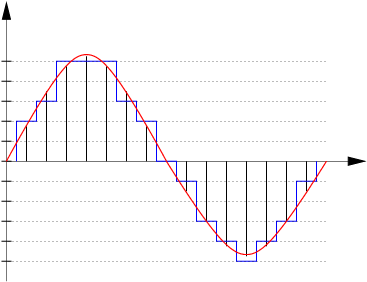
\includegraphics[scale=1]{S2IM1.png}
    \caption{Пример дискретизации звукового сигнала}
    \label{fig:section2:discrete}
\end{figure}

\subsection{Представление сигнала в виде спектрограммы}

Для использования методов машинного обучения в обработке звуковых и речевых сигналов
для получения более подробной информации о звуке, а также для более простого представления
звукового сигнала, звук представляют графически в виде спектрограмм.

Для введения понятия спектрограммы определим понятие спектральной плотности мощности звукового сигнала.

\emph{Спектральной плотностью мощности} в физике и теории обработки сигналов называется функция,
описывающая распределение мощности сигнала в зависимости от его частоты \cite{goldenberg}. 

Спектрограмма -- это изображение, которое показывает зависимость спектральной плотности мощности сигнала от времени.

Наиболее распространенным видом спектрограммы является двумерная диаграмма, по горизонтальной оси которой идет отсчет времени,
а по вертикальной -- отсчет частоты. Третье измерение спектрограммы, указывающее амплитуду, 
представляется интенсивностью или цветом каждой точки плоскости изображения.

\begin{figure}[h!]
    \centering
    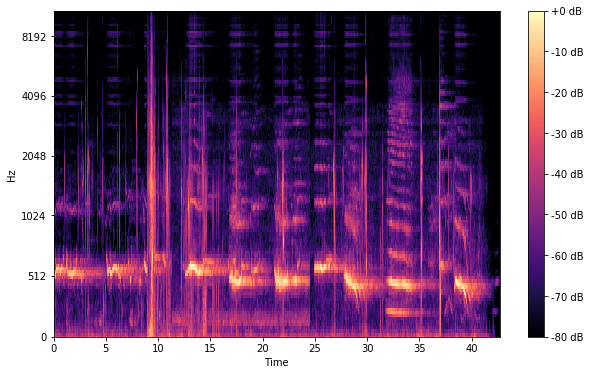
\includegraphics[scale=0.6]{S2IM2.png}
    \caption{Пример спектрограммы звукового сигнала}
\end{figure}

Получить спектрограмму звукового сигнала можно используя метод быстрого оконного преобразования Фурье,
который генерирует спектры за счет разделения исходного звукового сигнала на интервалы методом скользящего окна.